\documentclass[11pt]{article}
% Single-column readable draft (NOT the ACL two-column layout). To produce the
% camera-ready, swap the geometry/natbib block below back for
% \usepackage[review]{acl} and restore the \And author form.
\usepackage[margin=1.1in]{geometry}
\usepackage{times}
\usepackage{latexsym}
\usepackage[T1]{fontenc}
\usepackage[utf8]{inputenc}
\usepackage{microtype}
\usepackage{graphicx}
\usepackage{xcolor}
\usepackage{booktabs}
\usepackage{amsmath}
\usepackage{natbib}
\usepackage[hidelinks]{hyperref}
\setlength{\parskip}{0.4em}

% Resolve figures relative to this file (reports/) so includes find the repo dirs.
\graphicspath{{../}{../experiments/}{../img/}}

\newcommand{\am}[1]{\textcolor{orange}{[AM: #1]}}
\newcommand{\jb}[1]{\textcolor{blue}{[JB: #1]}} % draft notes / open items

\title{Read, Translate, Write: LLMs Translate with Fuzzy Semantic Hubs}
\author{First Author \and Second Author}

% =====================================================================
% DRAFT v5 (auto-assembled). Fleshes out the two empirical sections the
% intro promises: (1) the linear model from monolingual competence to
% translation (H1), and (2) GCM head/feature identification + the
% Multi-BLiMP head-ablation follow-up (H4). Intro/Related/§5(finetuning,
% H3, external) are kept as stubs -- copy the finished prose from v4.tex.
% Numbers are sourced from experiments/*/REPORT.md and the run outputs;
% see reports/P1_overview.md for the full provenance and validity flags,
% and PAPER_TODO.md for figures/items still pending.
% =====================================================================

\begin{document}
\maketitle
\begin{abstract}
\jb{Abstract last. One line: translation quality has strong separable
source/target structure, though the measured FLORES-perplexity linear fit is
weak (H1 caveat); the components that distinguish good from bad translations
overlap with sparse features the model uses to represent grammar monolingually
(H4); and collaborator-owned finetuning results should state H3 once verified.
Convergent, not conclusive, evidence that LLMs translate by reusing
language-modeling machinery through a multilingual ``semantic hub.''}
\end{abstract}

\section{Introduction}
\jb{Use the v4.tex introduction verbatim; it already states the stages-of-inference
framing and the three implications H1--H3 (and H4). Not reproduced here.}

\section{Related Work}
\jb{From v4.tex.}

% =====================================================================
\section{Monolingual Competence Predicts Translation Performance}
\label{sec:linear}

How much of a model's ability to translate is explained by its monolingual
language-modeling competence in the source and target languages, taken in
isolation? If translation reuses general language-modeling machinery, then a
model's BLEU on a language pair $(S,T)$ should be largely a function of two
monolingual quantities---competence in $S$ and competence in $T$---with no
language-pair-specific interaction term required (H1).

\paragraph{Setup.} For each ordered pair $(S,T)$ we fit the ordinary least
squares model
\begin{equation}
\hat{t}_{ST} = a + \beta_S\, l_S + \beta_T\, l_T,
\label{eq:linear}
\end{equation}
where $l_S, l_T$ is a monolingual-competence proxy for the source and target
language and $\hat t_{ST}$ is predicted BLEU; a bilinear variant adds an
interaction term $\beta_{ST}\, l_S l_T$, which under H1 should not help. We
compare proxies of two kinds: \emph{fluency} measures---corpus per-token
perplexity on FLORES devtest \citep{goyal2022flores}, and \emph{bits-per-byte}
(the same model NLL normalized by UTF-8 bytes rather than tokens, which removes
cross-lingual differences in tokenization granularity)---and a \emph{grammatical
acceptability} measure: MultiBLiMP accuracy \citep{jumelet2025multiblimp}, the
rate at which the model assigns higher probability to the grammatical member of
a minimal pair (equivalently $1-$PER, the perplexity-based version of the same
judgment). Fluency proxies cover all $24$ FLORES languages; MultiBLiMP covers
$17$, so the head-to-head comparison is on those $17$ ($272$ ordered
pairs).\footnote{BLEU provenance (companion \texttt{lang-similarity} repo,
\texttt{translation\_eval.py} $+$ \texttt{bleu\_similarity.py}): for each ordered
pair we prompt the base model 2-shot as \texttt{src$_1$ >> tgt$_1$|| src$_2$ >>
tgt$_2$|| src$_3$ >>} (two preceding FLORES sentences as in-context exemplars),
greedily decode up to $1.35\times$ the gold target's token length,
regex-extract the third \texttt{>>} segment, and score corpus BLEU
(\texttt{sacrebleu}) per direction over FLORES-101 \texttt{devtest}.
\jb{Confirm whether the canonical \texttt{bleu\_results.csv} used the committed
\texttt{devtest[:10\%]} slice or the full split.}}

\paragraph{Grammatical competence predicts BLEU; fluency does not.} All numbers
in this paragraph and in Table~\ref{tab:proxy} are computed on the common
$\mathbf{17}$-language set MultiBLiMP covers
(\texttt{ces, deu, ell, eng, fas, fra, heb, hin, ita, nld, pol, por, ron, rus,
spa, tur, ukr}; $272$ ordered pairs), so all proxies are compared on identical
data. The grammatical-acceptability proxy predicts BLEU with $R^2 = 0.25$ and
the correct sign (more accurate $\Rightarrow$ higher BLEU), weighting
target-language competence about $3.4\times$ the source ($\beta_T \approx 65$
vs.\ $\beta_S \approx 19$), with a significant per-language marginal relationship
(Spearman $\rho = +0.62$, $p = 0.008$ between a language's acceptability accuracy
and the mean BLEU into it; Fig.~\ref{fig:proxy}). The fluency proxies
\emph{fail}: per-token perplexity gives $R^2 = 0.07$ and bits-per-byte
$R^2 = 0.01$, both with the \emph{wrong} sign. Crucially, bits-per-byte removes
the cross-lingual tokenization confound that distorts per-token perplexity (e.g.\
English has higher per-token perplexity than Hebrew, the reverse of competence)
yet still carries no competence signal---so the failure is not a tokenization
artifact: monolingual \emph{fluency/compression} is simply not the quantity that
transfers to translation, whereas grammatical \emph{acceptability} is. The
bilinear (interaction) model does not improve on the linear one
(Table~\ref{tab:proxy}), consistent with H1's no-interaction prediction.

\begin{table}[t]
\centering
\small
\begin{tabular}{lccc}
\toprule
Model & $R^2$ & adj.\ $R^2$ & MAE \\
\midrule
MultiBLiMP accuracy --- linear   & \textbf{0.250} & 0.244 & 4.86 \\
MultiBLiMP accuracy --- bilinear & 0.251 & 0.243 & 4.84 \\
Per-token perplexity --- linear  & 0.071 & 0.064 & 5.43 \\
Bits-per-byte --- linear         & 0.012 & 0.005 & 5.49 \\
\bottomrule
\end{tabular}
\caption{Predictive power for translation BLEU, all on the same common $17$
MultiBLiMP languages (\texttt{ces, deu, ell, eng, fas, fra, heb, hin, ita, nld,
pol, por, ron, rus, spa, tur, ukr}; $272$ ordered pairs). MultiBLiMP accuracy
$\equiv$ perplexity-accuracy ($1-$PER), so the latter is not listed separately.
The bilinear model (interaction term) does not beat the linear one.}
\label{tab:proxy}
\end{table}

\begin{figure}[t]
\centering

\includegraphics[width=.82\linewidth]{outputs/perplexity_bleu_linear/competence_proxy_comparison/fig_multiblimp_marginal.png}
\caption{MultiBLiMP grammatical-acceptability accuracy vs.\ mean BLEU when
translating \emph{into} each language, over the $17$ MultiBLiMP languages
(\texttt{ces, deu, ell, eng, fas, fra, heb, hin, ita, nld, pol, por, ron, rus,
spa, tur, ukr}). Spearman $\rho=+0.62$ ($p=0.008$). Produced by
\texttt{compare\_competence\_proxies.py}.}
\label{fig:proxy}
\end{figure}

\paragraph{The BLEU surface is separable.} Independent of any proxy, we ask
whether the $(S,T)$ BLEU matrix $M$ itself factorizes into a source term and a
target term. We take its rank-1 SVD reconstruction $M_1$ and measure
$\text{faithfulness} = 1 - \lVert M - M_1\rVert_F / \lVert M\rVert_F$. A rank-1
matrix is exactly separable, $M_1(S,T)=f(S)g(T)$ (no pair-specific residual). We
find faithfulness $\mathbf{88.3\%}$ (Llama) and $82.4\%$ (Aya) on the
$24\times24$ matrix over all $24$ FLORES languages (the $17$ above plus
\texttt{ara, ind, jpn, kor, vie, zho\_simpl, zho\_trad}; the $24$ diagonal
self-cells are missing and imputed by column mean), robust to dropping any
single language (Llama leave-one-out $0.878$--$0.888$ vs.\ $0.883$ full). So
BLEU $\approx f(S)g(T)$: well approximated by separate source and target
factors, the structural form H1 predicts.

\begin{figure}[t]
\centering
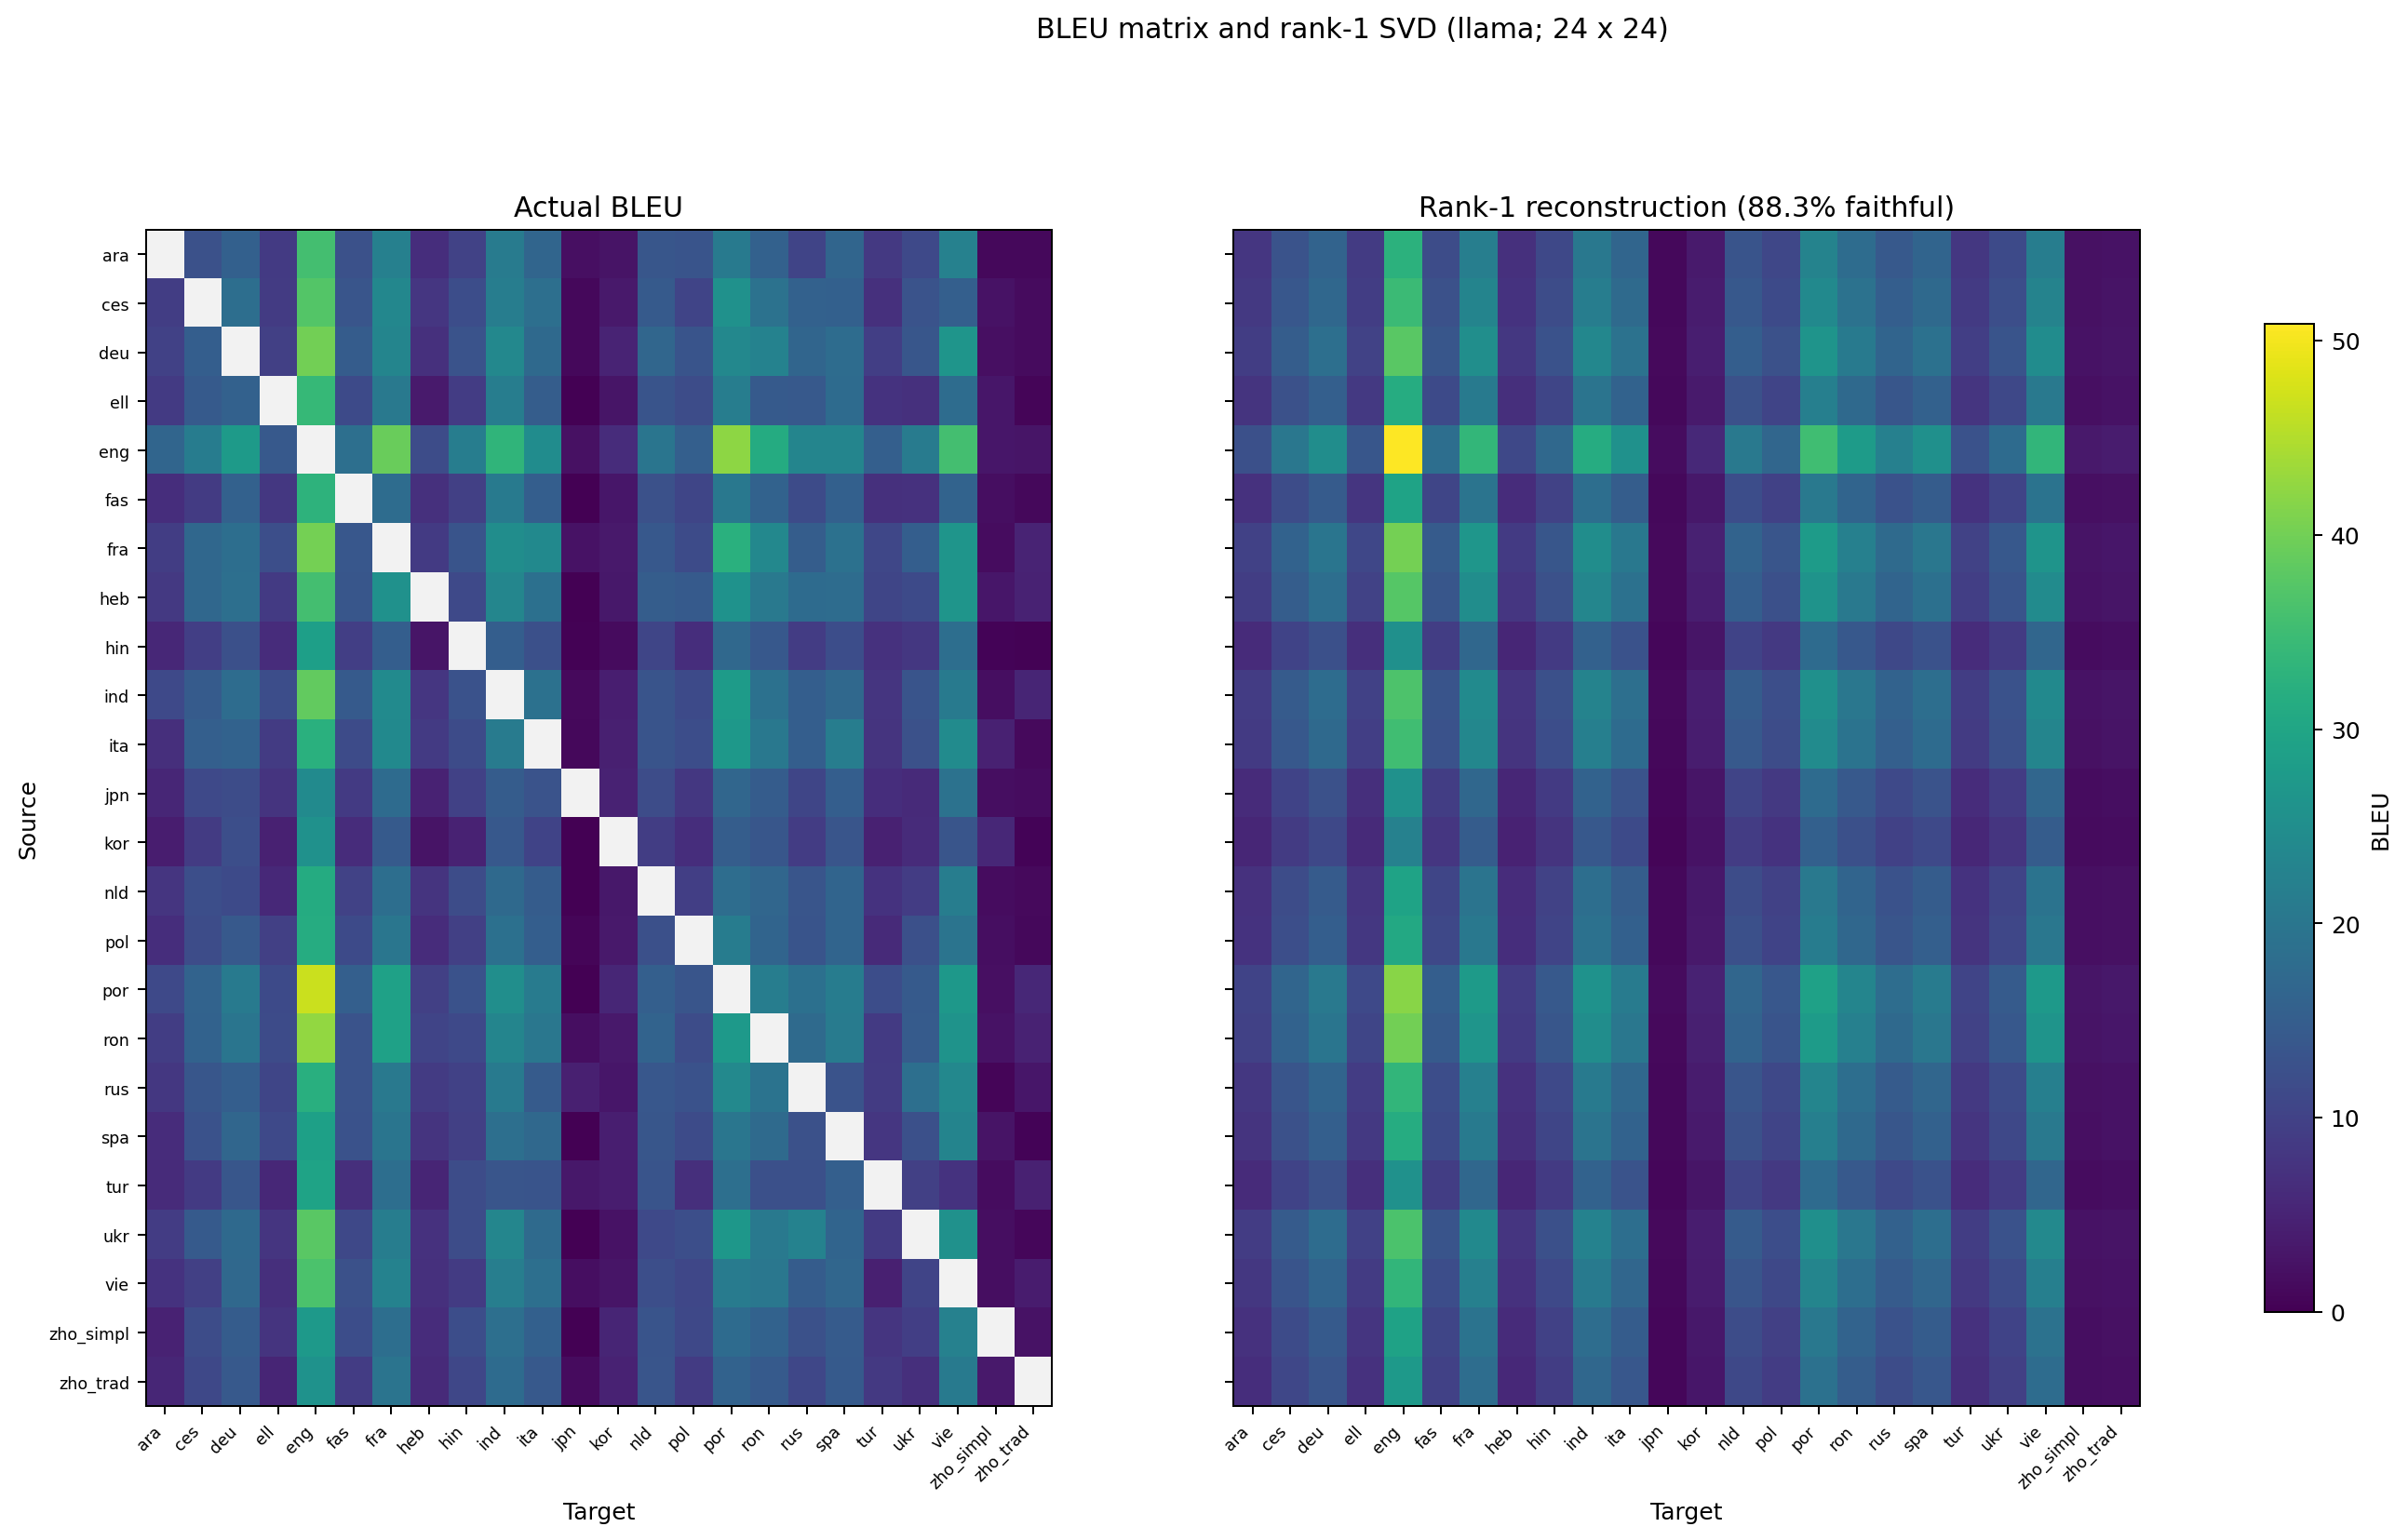
\includegraphics[width=\linewidth]{img/perplexity_bleu_linear/bleu_matrix_rank1_llama.png}
\caption{Raw Llama BLEU matrix and its rank-1 SVD reconstruction from the
\texttt{combined\_results\_llama.csv} pivot ($88.3\%$ faithful). $24\times24$;
$24$ missing self-cells imputed by target-column mean. Produced by
\texttt{rank1\_approximation.py}.
\jb{Mean-imputation can inflate the low-rank fit; a masked / observed-cells-only
recompute is the clean check (PAPER\_TODO A1).}}
\label{fig:rank1}
\end{figure}

Together these point the same way for H1: a monolingual grammatical-competence
proxy is a real, correctly-signed---if modest ($R^2\approx0.25$)---predictor of
translation quality, and the BLEU surface is structurally separable into source
and target factors with no pair-specific interaction. We do \emph{not} claim
perplexity is a usable competence measure; it is not.
\jb{Caveats: MultiBLiMP covers $17$ languages (European-heavy, no CJK), so the
head-to-head excludes the lowest-BLEU directions; $R^2{=}0.25$ is modest (MAE
$\approx4.9$ BLEU); MultiBLiMP acceptability and BLEU both reward well-formed
text, a mild shared-construct concern; bits-per-byte here is an exact algebraic
reconstruction from the saved per-token PPL (a direct $\sum\!\mathrm{NLL}/\sum\!\mathrm{bytes}$
GPU pass would reproduce it). Full analysis + per-language figures:
\texttt{reports/competence\_proxy\_comparison.md}.}

% =====================================================================
\section{Translation-Relevant Components Overlap With Language-Modeling Machinery}
\label{sec:gcm}

We now ask, mechanistically, \emph{which} model components carry the information
that distinguishes a correct translation from an incorrect one, and whether
those components are translation-specific or shared with monolingual language
modeling (H4). We proceed in two steps: (i) identify the influential components
with Generative Causal Mediation (GCM) on translation pairs
(\S\ref{sec:gcm-id}), then (ii) test whether the heads GCM implicates also carry
\emph{monolingual} grammatical information, by ablating them on Multi-BLiMP
minimal pairs (\S\ref{sec:gcm-ablate}).

\subsection{Identifying influential components with GCM}
\label{sec:gcm-id}

\paragraph{Background: indirect effects.} We want a \emph{causal} measure of how
much one internal component matters for the model's choice between two
translations. Fix a contrastive triple $(p_{\text{orig}}, r_{\text{orig}},
r_{\text{cf}})$---one prompt and two candidate continuations---and define the
preference metric
\begin{equation}
M = \log \pi(r_{\text{cf}}\mid p_{\text{orig}}) - \log \pi(r_{\text{orig}}\mid p_{\text{orig}}),
\label{eq:metric}
\end{equation}
where $\log\pi(r\mid p) = \sum_t \log p(r_t \mid p, r_{<t})$ is the
teacher-forced log-probability of a continuation, summed over its tokens (in
nats). $M$ is thus the model's log-odds preference for $r_{\text{cf}}$ over
$r_{\text{orig}}$ under the \emph{same} prompt. Now single out one component---an
attention head's output contribution, or one SAE feature---with activation $z$,
and write $M(z)$ for the metric as a function of that one activation while the
rest of the forward pass is held at its original-run values. The component takes
the value $z_{\text{orig}}$ on the original run and $z_{\text{cf}}$ on a run
where the model instead reads the counterfactual source. In the language of
causal mediation, the component is a \emph{mediator}, and its \emph{indirect
effect} is the change in $M$ caused by moving it between these two values---which
is exactly what activation patching measures, at a cost of one forward pass per
component:
\begin{equation}
\mathrm{IE}_{\text{patch}}(z) = M(z_{\text{orig}}) - M(z_{\text{cf}}).
\label{eq:patch}
\end{equation}

\paragraph{The GCM estimator.} GCM \citep{sankaranarayanan2026gcm} removes the
per-component cost by linearizing $M$ around $z_{\text{orig}}$. A first-order
Taylor expansion gives $M(z_{\text{cf}}) \approx M(z_{\text{orig}}) + \nabla_z
M|_{z_{\text{orig}}}\!\cdot(z_{\text{cf}} - z_{\text{orig}})$; substituting into
Eq.~\ref{eq:patch},
\begin{equation}
\widehat{\mathrm{IE}}(z) = \nabla_z M\big|_{z=z_{\text{orig}}} \cdot (z_{\text{orig}} - z_{\text{cf}}).
\label{eq:ie}
\end{equation}
This recovers $\mathrm{IE}_{\text{patch}}$ to first order but is computable for
\emph{every} component at once: the gradients $\nabla_z M$ come from a single
backward pass, and the deltas $(z_{\text{orig}} - z_{\text{cf}})$ from caching
each component's activation on the original and counterfactual runs. So one
forward$+$backward pass yields an IE estimate for all $1024$ heads and all
$32{,}768$ SAE features, versus one patched forward pass \emph{each} for the
exact version.

\paragraph{Reading magnitude and sign.} $\widehat{\mathrm{IE}}$ is in nats. Its
magnitude $|\widehat{\mathrm{IE}}|$ is how much the component, on its own, shifts
the preference between the two continuations; we rank components by
$\mathrm{mean}\,|\widehat{\mathrm{IE}}|$ over the $100$ pairs. Its sign---under
this orig-minus-cf convention, with $M = m_{\text{cf}} - m_{\text{orig}}$---says
which continuation the component favors in its original state: a positive
$\widehat{\mathrm{IE}}$ means the original activation (relative to the
counterfactual) pushes the model toward $r_{\text{cf}}$; a negative value means
it pushes toward the gold response $r_{\text{orig}}$. Section~\ref{sec:gcm-ablate}
turns on exactly this sign.\footnote{A first-order estimate is only as good as
the linearization. The repo's finite-difference test checks
$M(z_{\text{orig}}+\varepsilon\,\delta) - M(z_{\text{orig}}) \approx
\varepsilon\,\nabla_z M\cdot\delta$ per pair; it is currently \texttt{xfail}
(see PAPER\_TODO A2), so the linearization is taken on faith pending that check.}

\paragraph{Contrastive pairs from translation.} Rather than hand-written
contrasts, we use FLORES sentence pairs: $r_{\text{orig}}$ is the gold
translation of the original source, $r_{\text{cf}}$ the gold translation of a
different (counterfactual) source, both scored under the same prompt
$p_{\text{orig}}$. We attribute every attention head ($32\times32$ query-head
outputs, sliced from \texttt{o\_proj.input}) and every layer-16 SAE feature
($32{,}768$ features of \texttt{jbrinkma/sae-llama-3-8b-layer16}), patching at
the \emph{last source-token position} only. We sweep all $56$ ordered
cross-language directions among
\{eng, spa, deu, fra, tur, ara, hin, heb\}, nominally $100$ pairs per direction
(eng$\to$fra has $98$ successful pairs), on a 2-shot prompt.\footnote{Two
implementation points the method depends on: each
pair is scored in \emph{two} separate single-invoke traces (not one batched
multi-invoke trace, which left-pads and would shift the patched index); and
because writing to a module \emph{input} is unsupported, the per-head patch is
applied as the equivalent additive delta $(z-z_{\text{orig}})W_o^{\!\top}$ at
\texttt{o\_proj.output}.}

\paragraph{Control tasks.} The central methodological device is a $2\times2$
factorial that subtracts away two confounds---generic content discrimination
and cross-language routing---so the residual is attributable to a translation
circuit. The factors are \emph{cross} vs.\ \emph{same} (whether $S\!\neq\!T$, so
the model must route across languages) and \emph{real} vs.\ \emph{null} (whether
one scored response is the gold translation of the source, providing a
correctness anchor; in the \emph{null} condition both responses are gold
translations of \emph{other} sentences). The resulting subtractions are:
$\textsc{real\_cross}-\textsc{null\_cross}$ (translation-circuit-specific),
$\textsc{null\_cross}-\textsc{null\_same}$ (cross-language routing), and
$\textsc{real\_same}-\textsc{null\_same}$ (monolingual identity completion).
\textsc{null\_same}, where both responses are arbitrary same-language contents,
is the pure content-discrimination floor.

\paragraph{Sanity checks.} The identity patch ($z=z_{\text{orig}}$) reproduces
the unpatched metric to within bf16 round-off (drift $=0.0$ across all $56$
directions); the clean model prefers the gold over the counterfactual response
in $\geq99\%$ of pairs (length-normalized); and the top-$20$ head set is stable
under bootstrap resampling (inclusion frequency $0.92$--$1.00$). \jb{The
finite-difference linearization test is currently \texttt{xfail}, and the
ACP-vs-ATP interventional faithfulness check has not been run on the sweep; see
PAPER\_TODO A2.}

\paragraph{Result: heads look universal, but are mostly content.} Counting how
often each head lands in a direction's top-$20$, two heads (L17H21, L30H25)
appear in \emph{all $56$} directions, and the top-$20$ is dominated by late
layers (L28--L31); one SAE feature (f20383) is universal across all $56$
directions as well. Taken at face value this suggests shared ``universal
translation heads.'' The control tasks, however, substantially revise this
reading at the head level: the translation-circuit-specific contribution
$(\textsc{real\_cross}-\textsc{null\_cross})$ for the top heads is at most
$+0.025$ nat---at the bf16 noise floor. L30H25 is illustrative: its
$\textsc{real\_cross}$ effect ($+0.48$) is dwarfed by its $\textsc{null\_same}$
effect ($+1.21$), i.e.\ it fires \emph{more} in monolingual same-language
completion than in translation. At the head level it is a content head, not a
translation head. (The per-direction IE maps are nonetheless sparse and
structured, not uniform noise: the top-head/median-head mean-$|\widehat{\mathrm{IE}}|$
ratio runs $21.8$--$62.9$ across the $56$ directions, median $34.6$;
App.~Fig.~\ref{fig:ie-sparsity}.)

\paragraph{Result: the sparse-feature signal is cleaner.} The same
decomposition at the SAE-feature level separates better. Feature f31444 is
nearly silent in monolingual completion ($\textsc{null\_same}=0.0004$) but has
substantial cross-language signal ($\textsc{real\_cross}=0.0741$,
$\textsc{null\_cross}=0.0380$), so about half ($+0.0361$ nat) is
translation-circuit-specific---the cleanest translation-relevant component we
find. Moreover, of the $50$ most direction-universal SAE features, $9$ also
belong to an independently-defined set of grammatical-concept features
(\S\ref{sec:gcm-ablate} \jb{/ cross-ref the input-feature work}), versus
$\approx0.33$ expected by chance---a $\sim$27$\times$ enrichment. The features
the model relies on to translate are disproportionately the same features it
uses to represent grammar monolingually, consistent with a shared multilingual
``semantic hub'' (H4/H2).

\begin{figure}[t]
\centering

\includegraphics[width=\linewidth]{experiments/gcm_translation/img/three_way_decomposition_sae_full.png}
\caption{SAE-feature three-way decomposition. Per top feature, the mean
$|\widehat{\mathrm{IE}}|$ under \textsc{real\_cross}, \textsc{null\_cross}, and
\textsc{null\_same}, and the derived translation-circuit contribution. f31444 has
$\textsc{null\_same}\approx0$. Produced by \texttt{three\_way\_decomposition.py}
(full view: 56 cross-lang $+$ 8 same-lang directions).
\jb{Foreground the SAE figures over the head version (the head one is at the
noise floor); a head companion can go to the appendix. See PAPER\_TODO A2.}}
\label{fig:gcm-decomp}
\end{figure}

\begin{figure}[t]
\centering
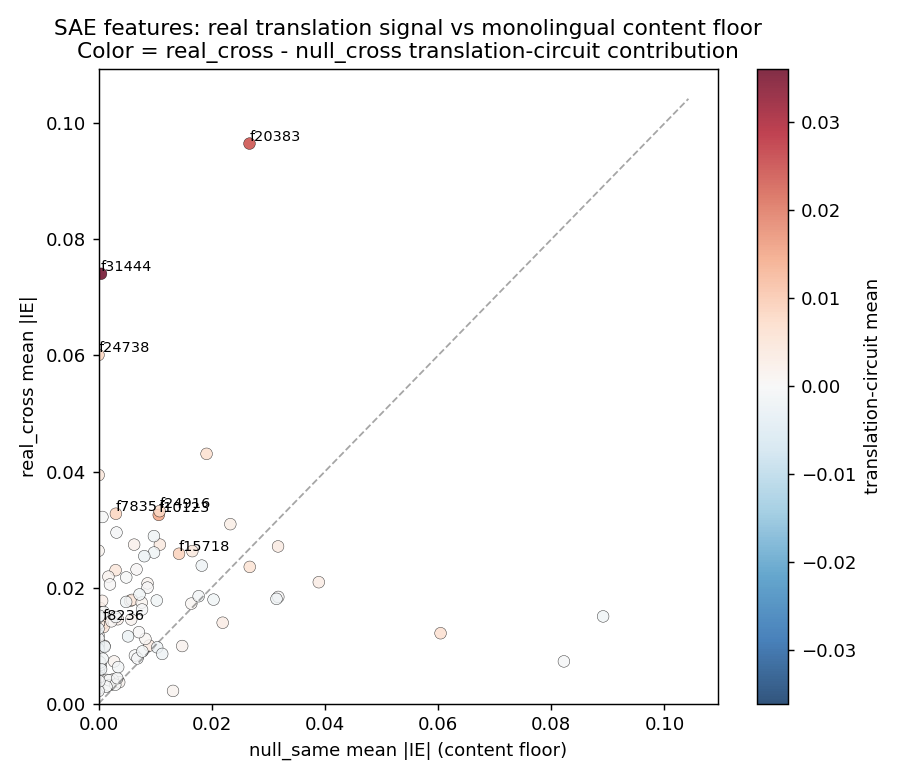
\includegraphics[width=\linewidth]{experiments/gcm_translation/img/meeting_sae_real_vs_null_same.png}
\caption{Per SAE feature, the real (\textsc{real\_cross}) mean
$|\widehat{\mathrm{IE}}|$ against the content-discrimination floor
(\textsc{null\_same}). Features far below the diagonal---most notably f31444---are
active in translation but silent in monolingual same-language completion, i.e.\
translation-circuit-specific rather than pure content. Produced by
\texttt{meeting\_plots.py} from the three-way summary.}
\label{fig:gcm-sae-realnull}
\end{figure}

\begin{figure}[t]
\centering

\includegraphics[width=\linewidth]{experiments/gcm_translation/img/meeting_sae_grammar_overlap.png}
\caption{The $50$ most direction-universal layer-16 SAE features, by number of
the $56$ directions in which each appears in the top-$20$; red bars mark
features that also belong to the grammar-feature set ($9/50$ overlap vs.\
$\approx0.33$ by chance). Produced by \texttt{meeting\_plots.py} from the
cross-direction aggregation in \texttt{analyze.py}.}
\label{fig:gcm-grammar}
\end{figure}

\begin{figure}[t]
\centering
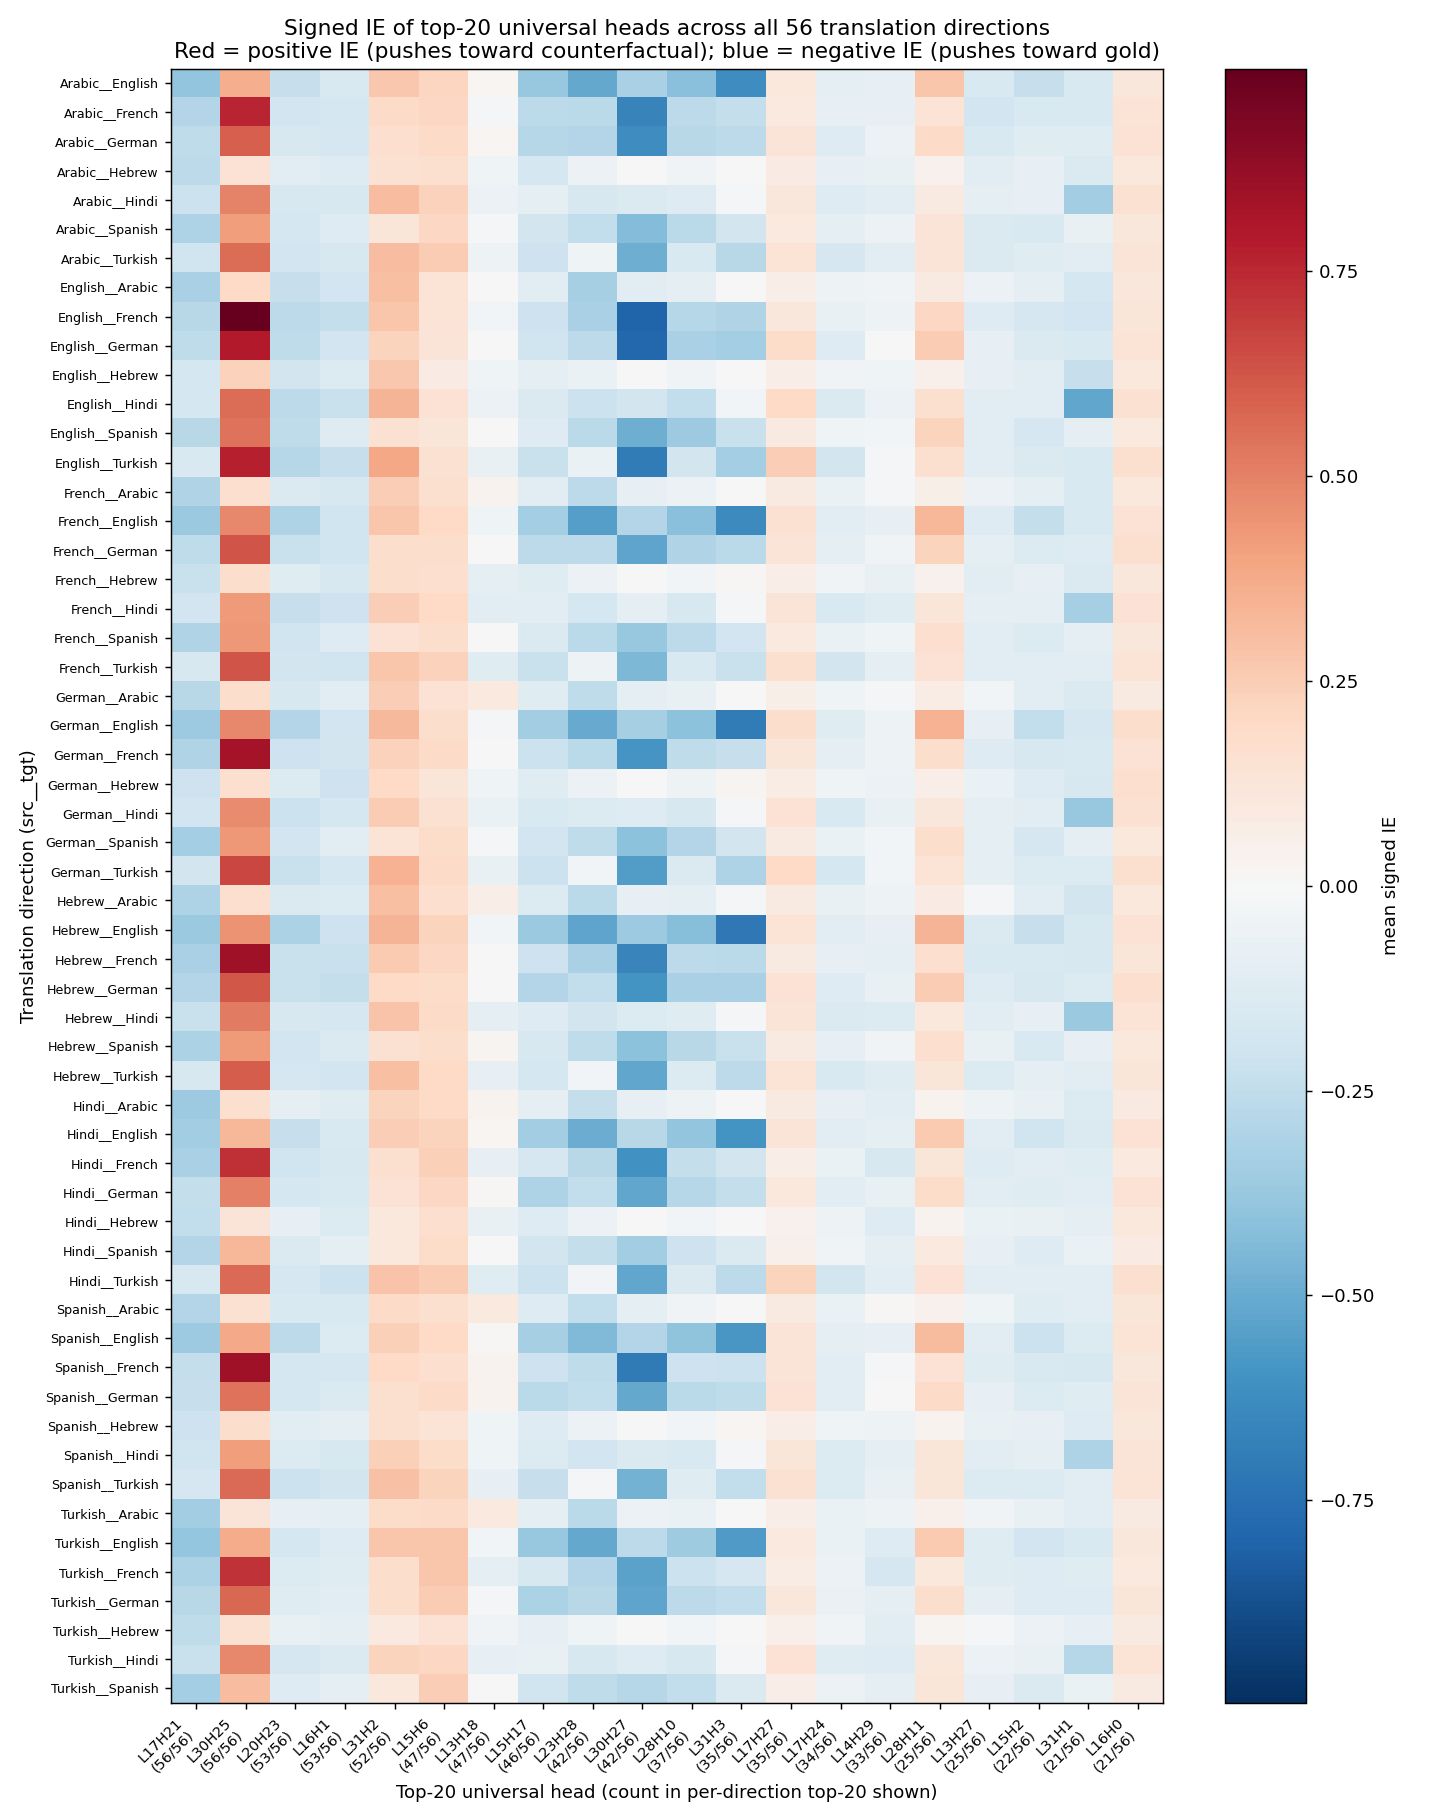
\includegraphics[width=\linewidth]{experiments/gcm_translation/img/meeting_direction_by_universal_head_signed.png}
\caption{Signed IE of the top-$20$ universal heads across all $56$
cross-language directions ($K{=}20$, from
\texttt{analyze.py --top\_k\_for\_universality 20}). Red cells indicate positive
IE (the head's original state pushes toward the counterfactual response); blue
cells indicate negative IE (pushes toward the gold response). The plot makes the
head-level caveat visible: high reuse counts do not imply translation-specificity
after the null controls (cf.\ Fig.~\ref{fig:gcm-decomp}). Produced by
\texttt{meeting\_plots.py}.}
\label{fig:gcm-signed-heads}
\end{figure}

\subsection{Signed GCM head groups predict monolingual grammatical effects}
\label{sec:gcm-ablate}

If translation reuses language-modeling machinery, the heads GCM implicates for
\emph{translation} should also matter for \emph{monolingual} grammaticality.

\paragraph{Method.} For each target language $L$ we aggregate GCM head effects
over the seven directions \emph{into} $L$ (excluding $L\!\to\!L$), taking the
per-pair mean of both $|\widehat{\mathrm{IE}}|$ and signed
$\widehat{\mathrm{IE}}$, and select the top-$20$ heads by aggregated mean
absolute IE. We then split this set by the sign of the aggregated signed IE into
a \textsc{pos} and a \textsc{neg} sub-population. We score each Multi-BLiMP
minimal pair by $\Delta = \log p(\text{correct final token}) -
\log p(\text{incorrect final token})$ at the prefix-final position, and report
$\Delta_{\text{change}} = \Delta_{\text{ablation}} - \Delta_{\text{baseline}}$
under mean-ablation of a head set (replacing the head's \texttt{o\_proj.input}
slice with its position-averaged language mean, applied via the equivalent
output delta). A negative $\Delta_{\text{change}}$ means ablation weakened the
grammaticality margin; positive means it strengthened it. Controls are
stratified same-layer random heads. We run six languages at $n{=}400$ and two
(heb, hin) at $n{=}200$.

\paragraph{Result: GCM sign predicts the monolingual ablation effect.} In all
eight languages, ablating the \textsc{neg}-signed sub-population
\emph{weakened} the grammaticality margin ($\Delta_{\text{change}}$ from $-0.12$
to $-1.02$), while ablating the \textsc{pos}-signed sub-population
\emph{strengthened} it ($+0.05$ to $+0.22$). A property measured purely in the
translation task---the sign of a head's GCM indirect effect---thus predicts the
direction of its causal effect on a monolingual grammaticality task. The
\textsc{neg}-signed heads (the majority, $\sim$65--80\% of the top-$20$) behave
like shared language-modeling machinery that translation borrows; the smaller
\textsc{pos}-signed population behaves like translation-specific routing, whose
removal does not carry monolingual grammaticality information. By contrast, the
mixed top-$5$ collective and the random controls are at the noise floor in
$7/8$ languages, because a set chosen by absolute IE alone mixes the two
opposing populations. For the one language with size-matched controls so far
(English---the only completed $53$-condition v2 run), the matched-size POS/NEG
random controls sit near zero ($-0.028$, $+0.032$) while the sign-split groups
are several times larger ($+0.075$, $-0.160$), an early sign that the effect is
not a group-size artifact; matched controls for the other seven languages are
queued (job \texttt{5772145}, n=400, A100).

\begin{figure}[t]
\centering
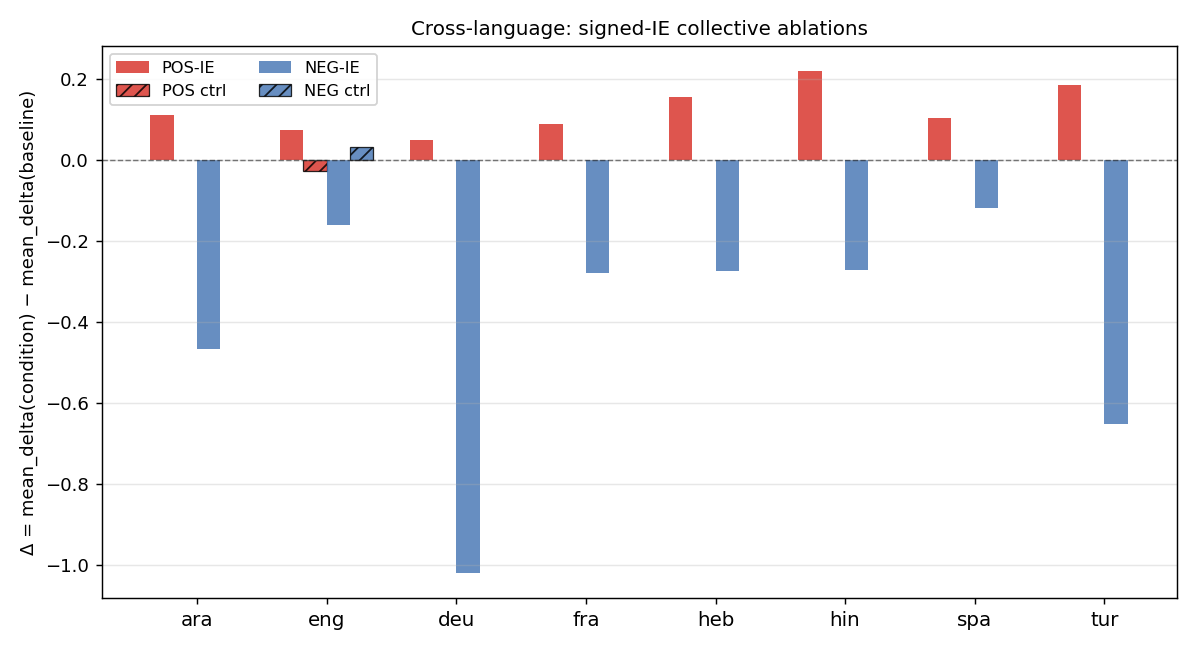
\includegraphics[width=\linewidth]{experiments/head_ablation_multiblimp/img/cross_lang_sign_split.png}
\caption{Per-language $\Delta_{\text{change}}$ on Multi-BLiMP from ablating the
\textsc{pos}-signed vs.\ \textsc{neg}-signed sub-population of the top-$20$ GCM
heads. Negative means ablation weakened the grammaticality preference. Produced
by \texttt{visualize.py} from \texttt{analysis\_summary.csv}.
\jb{Size-matched controls exist for English only so far; the 7-language rerun is
queued (job \texttt{5772145}). Regenerate this figure once it lands. Full
per-condition table $\to$ appendix; see PAPER\_TODO A3.}}
\label{fig:ablate-signsplit}
\end{figure}

\jb{Open caveats to fold into Limitations: (i) head-level translation-circuit
contributions in \S\ref{sec:gcm-id} are at the bf16 noise floor---the
feature-level evidence is the stronger claim; (ii) head selection here uses the
pre-control Phase-1 ranking; (iii) several $\Delta_{\text{change}}$ values are
within 2--3$\times$ of the noise floor; (iv) heb/hin at $n{=}200$; (v) the
size-matched sign-split controls are pending.}

% =====================================================================
\section{Monolingual Finetuning Is Competitive With Parallel Corpora}
\label{sec:finetune}
\jb{External (Jannik). Prose + figures to be supplied; states H3.}

\section{Discussion and Conclusions}
\jb{From v4.tex: the three results are convergent, not conclusive, evidence that
translation reuses language-modeling machinery through a multilingual semantic
hub. Emphasize that translation-selective mechanisms surely also exist; our aim
is to explain why monolingual pretraining helps translation at all.}

\section*{Limitations}
\jb{All interpretability results are Llama-3.1-8B with a single layer-16 SAE on a
base (non-instruction-tuned) model; Aya appears only in \S\ref{sec:linear}.
Plus the head-level / noise-floor / sample-size caveats noted above. The H2
input-output overlap result is also weak in the current saved outputs: across
the 25 cells with usable vectors, mean Jaccard@200 is only 0.095 using raw
scores and 0.122 using absolute-magnitude scores; several cells are missing or
malformed.}

\bibliographystyle{acl_natbib}
\bibliography{custom}
% Bib keys to add: sankaranarayanan2026gcm (arXiv:2602.16080),
% goyal2022flores, jumelet2025multiblimp.

\appendix
\section{Supplementary figures}

\begin{figure}[h]
\centering
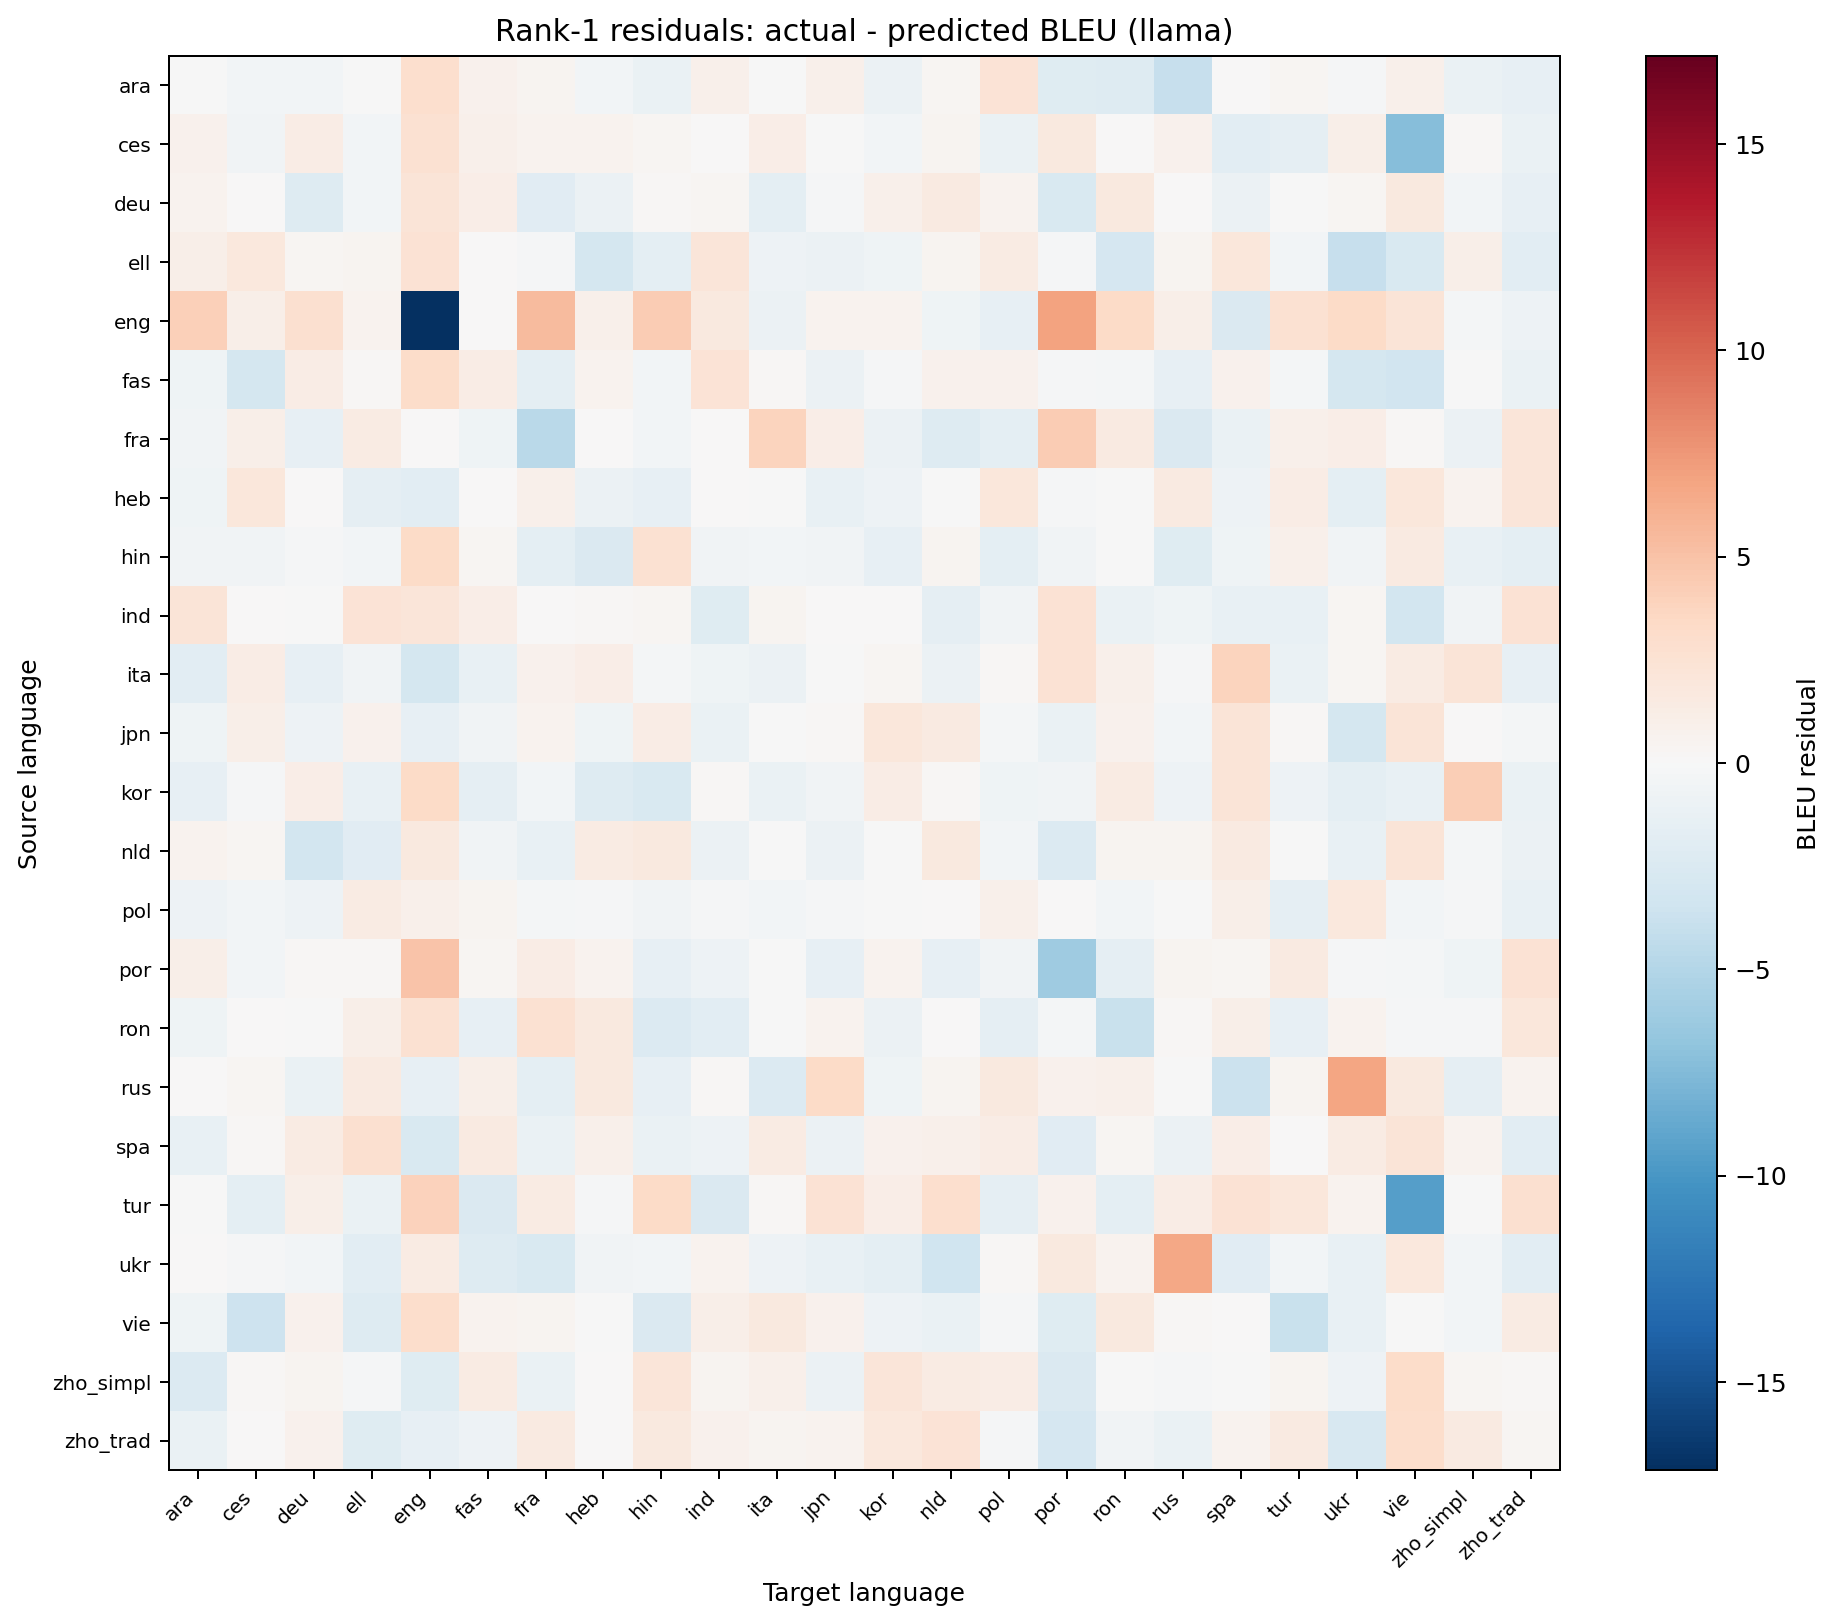
\includegraphics[width=.8\linewidth]{img/perplexity_bleu_linear/rank1_residual_heatmap_llama.png}
\caption{H1: residual of the rank-1 reconstruction of the Llama BLEU matrix
(actual $-$ rank-1), per (source, target). Produced by
\texttt{rank1\_approximation.py}.}
\label{fig:rank1-resid}
\end{figure}

\begin{figure}[h]
\centering
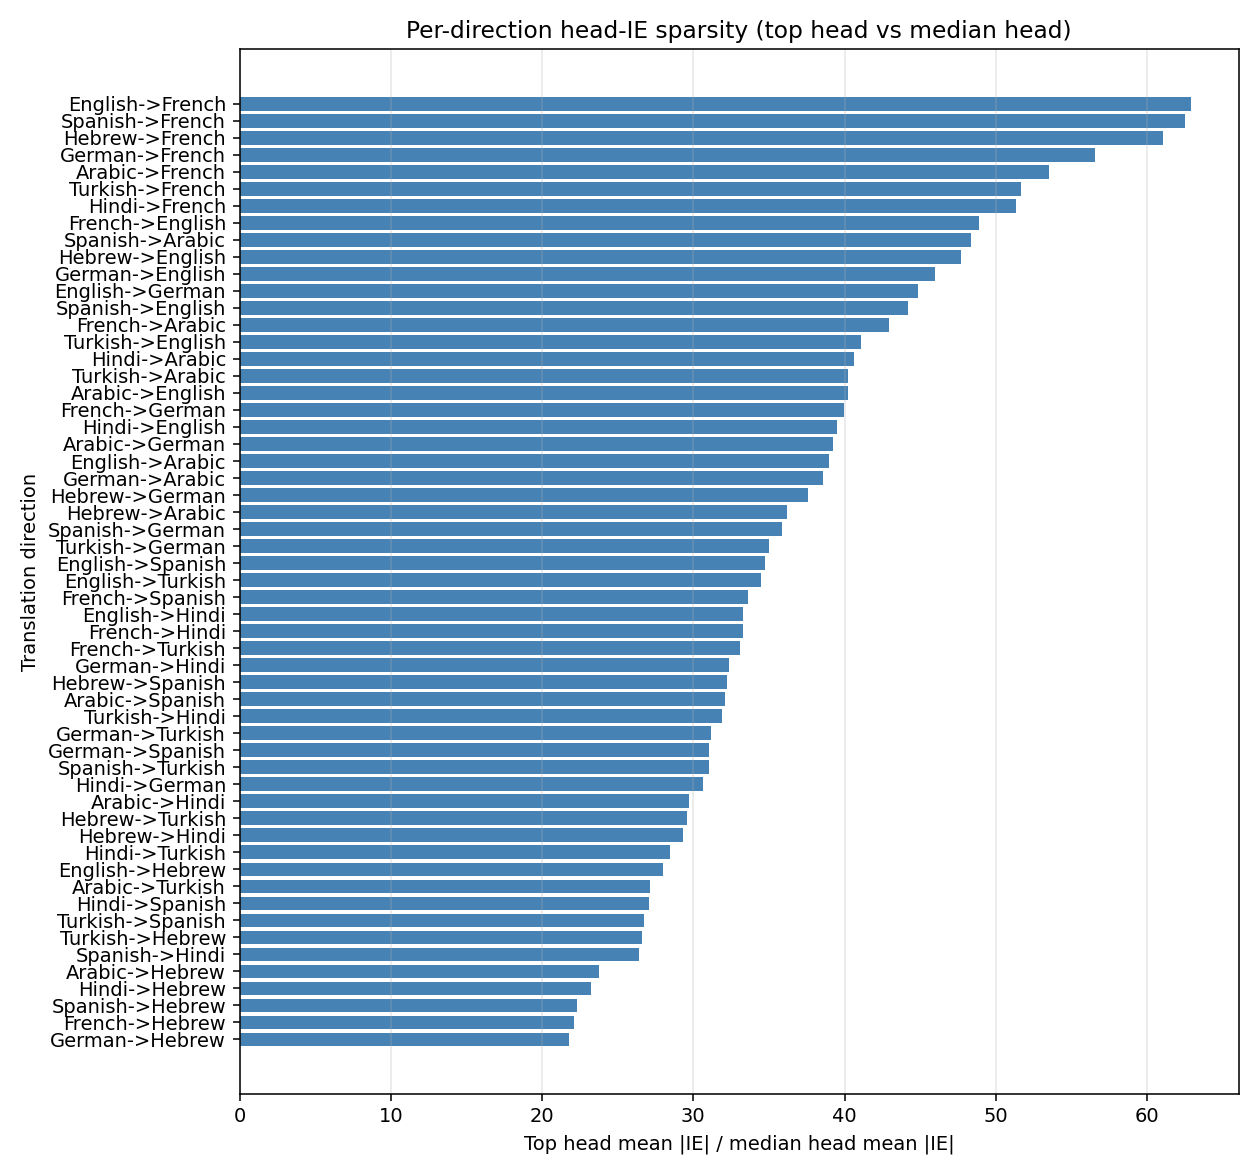
\includegraphics[width=.8\linewidth]{experiments/gcm_translation/img/head_ie_top_median_ratio.png}
\caption{GCM head-IE sparsity: per-direction top-head/median-head mean
$|\widehat{\mathrm{IE}}|$ ratio across the $56$ cross-language directions (range
$21.8$--$62.9$, median $34.6$). Produced by \texttt{summarize\_ie\_sparsity.py}.}
\label{fig:ie-sparsity}
\end{figure}

\begin{figure}[h]
\centering
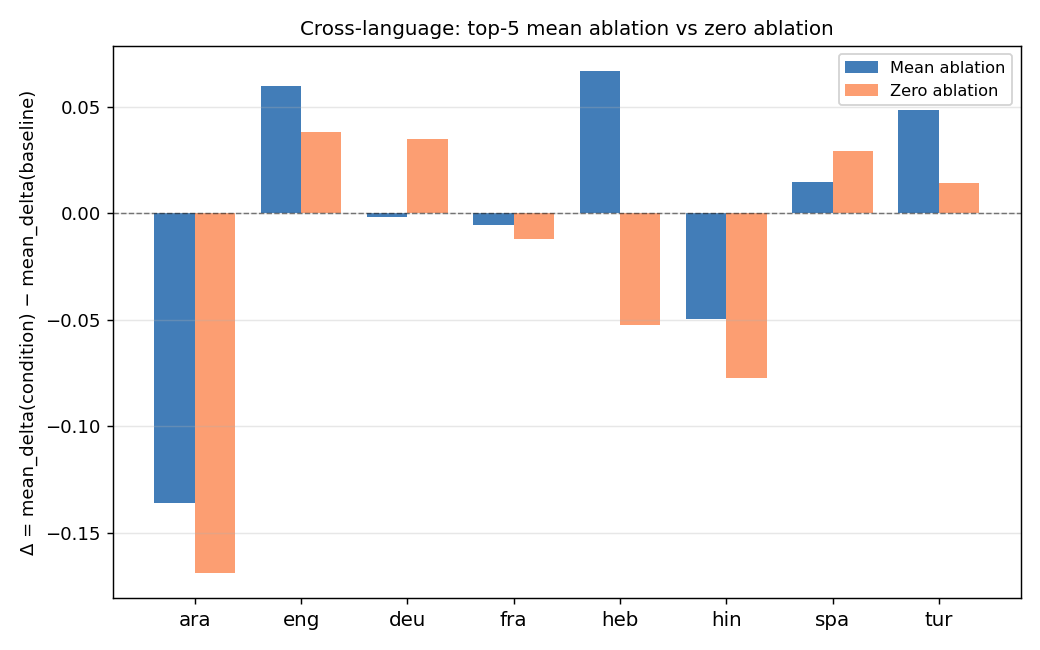
\includegraphics[width=\linewidth]{experiments/head_ablation_multiblimp/img/cross_lang_mean_vs_zero.png}
\caption{Head ablation: mean-ablation versus zero-ablation for the top-$5$
GCM-head collective across target languages.}
\end{figure}

\begin{figure}[h]
\centering

\includegraphics[width=.49\linewidth]{experiments/gcm_translation/img/heads_heatmap/English__Spanish_heads_heatmap.png}

\includegraphics[width=.49\linewidth]{experiments/gcm_translation/img/heads_signed_heatmap/English__Spanish_heads_signed_heatmap.png}
\caption{Method illustration for English$\to$Spanish GCM: mean
$|\widehat{\mathrm{IE}}|$ over heads (left) and signed mean IE (right).}
\end{figure}

\jb{Full per-condition table: \texttt{analysis\_summary.csv} in the head-ablation
output dir; convert to a LaTeX table after the queued matched-control rerun.}

\end{document}
